\graphicspath{{../05QuantumPhysics/pics/}}

\chapter{Quantum Physics}\label{ch:QuantumPhysics}
\lettrine[lines=2]{\color{darkocre}T}{he} first type of operators -- and
corresponding tensors -- that we encountered has a simple type:
\[
\op{L}\,\vec{a} = \vec{b}\,.
\]
It is a linear unary function mapping vectors into vectors.


\begin{myprereq}{Prerequisite Knowledge}
To fully understand the material of this chapter, readers should be comfortable with the following concepts:

\begin{itemize}
	\item \phantom{phantom}
	\vspace{-0.5cm}
	\item State
	\item Dynamical equations
\end{itemize}	
\end{myprereq}

\section{Quantum System}\label{sec:QuantumSystem}
We are looking for a binary operator $\op{\sigma}$ that yields a number
based on two vectors:
\[
\ketbra{\sigma}{\sigma}\,\vec{a}\,\vec{b}=x\,.
\]

\section{Quantum State}\label{sec:QuantumState}
We are looking for a binary operator $\op{\sigma}$ that yields a number
based on two vectors:
\[
\ketbra{\sigma}{\sigma}\,\vec{a}\,\vec{b}=x\,.
\]
\subsection{States Overlap}
\[
\braket{\psi}{\phi}.
\]

\section{Quantum Dynamics}\label{sec:QuantumDynamics}
We are looking for a binary operator $\op{\sigma}$ that yields a number
based on two vectors:
\[
\ketbra{\sigma}{\sigma}\,\vec{a}\,\vec{b}=x\,.
\]

\section{Quantum Hamiltonian}\label{sec:QuantumHamiltonian}
We are looking for a binary operator $\op{\sigma}$ that yields a number
based on two vectors:
\[
\ketbra{\sigma}{\sigma}\,\vec{a}\,\vec{b}=x\,.
\]


\section{Quantum Bit}\label{sec:Qubit}
Any quantum system with two active states is called a \emph{qubit}. The state with lower energy is usually called \emph{ground state} and denoted as $\ket{g}$ or $\ket{0}$ (zero). The state with higher energy is usually called \emph{excited state} and denoted as $\ket{e}$ or $\ket{1}$ (one). The notation $\ket{0}\,,\ket{1}$ is used in the field of quantum information and computation.

If the energy of the ground and excited states are $E_g$ and $E_e$, respectively, then the Hamiltonian of a qubit can be written using projectors
\[
\op{H} = E_g\ketbra{g}{g}+E_e\ketbra{e}{e}\,.
\]
It requires an energy $\Delta E=E_e-E_g$ to excite the qubit from the lower energy state to the higher energy state. This energy may come from a quantum of electromagnetic field oscillating with frequency $\omega=\Delta E/\hbar$.

\subsection{Flipping Operator}
Transition between the states of a qubit can be described mathematically using operators that map one state into another. For example, an operator $\op{F}$ that \emph{flips} states must do the following:
\[
\op{F}\,\ket{0}=\ket{1}\,,\quad \op{F}\,\ket{1}=\ket{0}\,.
\]
Such operator can be easily built from the tensor products:
\[
\op{F} = \ketbra{1}{0}+\ketbra{0}{1}\,.
\]
Each term in this sum is useful in quantum theory. The first term is called \emph{raising operator} and is denoted as 
$ \op{\sigma}_\plus=\ketbra{1}{0}$. The second term is called \emph{lowering operator} and is denoted as $ \op{\sigma}_\minus=\ketbra{0}{1}$. Apparently, the raising operator excites the qubit from the ground state, while the lowering operator brings the qubit down from the excited state.

\begin{exercise}
	Calculate (a) $\op{\sigma}_\plus \op{\sigma}_\plus$; (b) $\op{\sigma}_\minus \op{\sigma}_\minus$; (c) $\op{\sigma}_\plus \op{\sigma}_\minus$; (d) $\op{\sigma}_\minus \op{\sigma}_\plus$.
\end{exercise}

\begin{exercise}
	Show that  $\op{\sigma}_\plus \op{\sigma}_\minus+\op{\sigma}_\minus \op{\sigma}_\plus=\op{I}$, where $\op{I}$ is the identity operator.
\end{exercise}

\begin{exercise}
	Show that the qubit Hamiltonian can be written in terms of the raising and lowering operators as follows:
	
	\[
	\op{H} = \hbar\omega\left(\op{\sigma}_\plus \op{\sigma}_\minus+\epsilon\op{I} \right)\,,
	\]
	where $\epsilon=E_g/\Delta E$.
\end{exercise}

\subsection{Number Operator}
The operator $\op{n}=\op{\sigma}_\plus \op{\sigma}_\minus$ is called \emph{number operator} for the following reason. First, note that $\op{\sigma}_\plus \op{\sigma}_\minus=\ketbra{1}{1}$ is the projector on the excited state of qubit.
 

\section{Quantum Oscillator}\label{sec:QuantumOscillator}
The \emph{principle of the quantization of action} can be applied to harmonic oscillator. The result is the quantization of energy levels. 

The energy of a harmonic oscillator can be expressed in terms of the maximum momentum $p_m$ or in terms of the maximum displacement $x_m$:
\[
H = \frac{p_m^2}{2m}\quad\textrm{ or }\quad H=\frac{kx_m^2}{2}\,.
\]
Multiplying these two equalities and recalling that $\omega^2=k/m$, we obtain
\[
H = \frac{\omega x_m p_m}{2}\,.
\]
The path which the state vector $\ket{\xi}=(x,p)$ follows in phase space is an ellipsis with the major semi-axes $x_m$ and $p_m$. The area of this ellipsis is $A=\pi x_m p_m$. Therefore, the connection between the energy of harmonic oscillator and the area is given by
\[
H=\frac{\omega}{2\pi}A\,.
\]
The area $A$ is a physical quantity with the units of action.

As shown in Figure \ref{fig:phaseSpaceQuantum}(a), areas in phase space have the smallest size limited by the elementary quantum of action $h$ -- known as Planck constant. The quantization of action and, consequently, the quantization of phase-space area, has two important implications for harmic oscillator.
\begin{figure}[htbp]
	\centering
	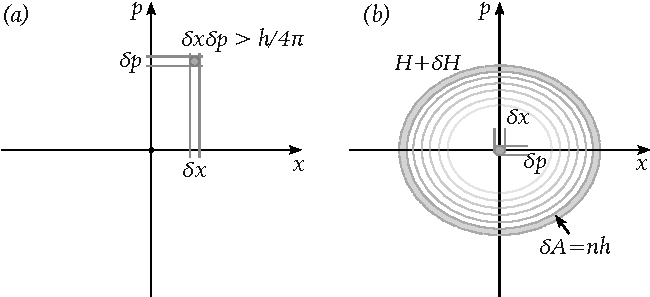
\includegraphics[scale=1.0]{phaseSpaceQuantum}
	\caption{Areas of phase-space regions have the units of action. Quantization of action implies quantization of phase-space area. (a) The smallest area in phase space is limited by the fundamental quantum of action $h$ -- Planck's constant. (b) Area of the ellipsis inside the path of harmonic oscillator is proportional to its energy. Quantization of area leads to the quantization of energy of harmonic oscillator.}
	\label{fig:phaseSpaceQuantum}
\end{figure}

First, every time an oscillator absorbs some energy $\Delta E$, the maximum deviation and the maximum momentum increase. The ellipsis in phase space increases its area. But since the area in phase space can't grow continiously--changes in discrete quanta $\delta A=h$--we must have discreete changes in energy. Second, the existence of the elementary quantum of action and the smallest are in phase space, require that the lowest energy state of harmonic oscillator is described not by a point in phase space, but by an elementary ellipsis such that $A_0=\delta x\delta p\propto h$. Putting these two ideas together, we conclude that the area of the ellipsis can be written as
\[
A_n = A_0 + nh\,.
\]
The energy of the oscillator then takes the form
\[
H=n\hbar\omega + E_0\,,
\]
where $\hbar=h/2\pi$ is called \emph{reduced Planck's constant}, and $E_0$ is the lowest energy of the harmonic oscillator. From the expression for $H$ follows that harmonic oscillator can be in a countable set of states, growing in energy from $E_0$ by a fixed step $\hbar\omega$. 

The energy of the lowest state can be written in terms of the step size $\hbar\omega$: $E_0=e_0\hbar\omega$, where $e_0$ is some number (it will be found later). Finally, we can write the energy of harmonic oscillator as follows:
\[
H=\hbar\omega(n + e_0)\,.
\]

\subsection{Hamiltonian Operator}
For any quantum system with descrete energy states $E_0, E_1, E_2,\ldots, E_n\ldots$ the Hamiltonian operator can be written in terms of projectors:
\[
\op{H}=\int E_k\ketbra{k}{k}\,,\quad k=0,1,2,\ldots,n\ldots 
\]
For harmonic oscillator $E_k=E_0+k\hbar\omega$ for $n>1$ and the Hamiltonian operator can be written as follows
\[
\op{H} = \int (E_0+k\hbar\omega)\ketbra{k}{k}\,.
\]
The number $k$ tells how many excitations quantum oscillator absorbed to reach the energy state $\ket{k}$.
Opening the parentheses and recalling that
\[
\int\ketbra{k}{k}=\op{I}\,,
\] 
we obtain 
\[
\op{H} = E_0\op{I}+\hbar\omega \int k\ketbra{k}{k}\,.
\]
This expression is very similar to the Hamiltonian of a qubit 
\[
\op{H}_{qb}=E_g\op{I}+\hbar\omega\op{n}
\]
where $\op{n}=\op{\sigma_\plus}\op{\sigma_\minus}$ is a number operator. The similarity is not accidental, as the operator $\op{n}=\int k\ketbra{k}{k}$ plays the role of the number operator. Indeed, it is easy to check by direction application that:
\[
\op{n}\,\ket{n}=n\ket{n}\,.
\]
In other words, the energy states $\ket{n}$ of harmonic oscillator, are the eigen-states of the number operator $\op{n}$ with the eigen-value $n$ corresponding to the number of excitation level.
\begin{exercise}
	Prove that $\op{n}\,\ket{n}=n\ket{n}$ by direction application of the operator $\op{n}=\int k\ketbra{k}{k}$.
\end{exercise}

The expression for the number operator $\op{n}$ can be obtained in a different way. First note that
\[
\op{H}\,\ket{n}=E_n\ket{n}\,,\quad\textrm{ where } E_n = E_0 + n\hbar\omega\,.
\]
From this follows
\[
(\op{H}-E_0\op{I})\,\ket{n}=n\hbar\omega\,\ket{n}\,,
\]
and, consequently, 
\[
\frac{(\op{H}-E_0\op{I})}{\hbar\omega}\,\ket{n}=n\,\ket{n}\,.
\]
The operator on the left hand side of this equation is the number operator $\op{n}$. It can be simplified once we recall that
\[
\op{H}=\int E_k\ketbra{k}{k}\quad\textrm{ and }\quad \op{I}=\int\ketbra{k}{k}\,.
\]
Using these relations, we first write
\[
\op{H}-E_0\op{I}=\int (E_k-E_0)\ketbra{k}{k}\,.
\]
Then, remembering that $E_k=E_0+k\hbar\omega$, we immediately arrive at
\[
\op{n}=\frac{(\op{H}-E_0\op{I})}{\hbar\omega}=\int k\ketbra{k}{k}\,.
\]
Thus, the operator of quantum harmonic oscillator can be written in the following form:
\[
\op{H}_{osc}=E_0\op{I}+\hbar\omega\op{n}\,.
\]
\subsection{Ladder Operators}
The number operator for qubit could be expressed as the product of two simple operators that raised or lowered qubit states:
\[
\op{n} = \op{\sigma}_\plus\op{\sigma}_\minus\,.
\]
The idea of raising and lowering states is also applicable to harmonic oscillator. Similar to qubit, we can write such operators as tensor products:
\[
\op{a}_\plus = \ketbra{n+1}{n}\textrm{ and }\quad\op{a}_\minus=\ketbra{n-1}{n}\,.
\]
Unfortunately, these operators will act properly only on the state $\ket{n}$.
\begin{exercise}
	Evaluate (a) $\op{a}_\plus \,\ket{n}$; (b) $\op{a}_\minus \,\ket{n}$; (c) $\op{a}_\plus \,\ket{n+m}$; (d) $\op{a}_\plus \,\ket{n+m}$.
\end{exercise}
It is easy to fix this problem by summing over all states:
\[
\op{a}_\plus=\int \ketbra{k+1}{k}\quad\textrm{ and }\quad \op{a}_\minus=\ketbra{0}{0}+\int \ketbra{m-1}{m}\,,\quad m > 0\,.
\]
The first term in the expression for $\op{a}_\minus$ ensures that the vacuum state remains unchanged: $\op{a}_\minus\,\ket{0}=\ket{0}$.
\begin{exercise}
	Evaluate (a) $\op{a}_\plus \,\ket{n}$; (b) $\op{a}_\minus \,\ket{n}$.
\end{exercise}
Let's check whether $\op{a}_\plus\op{a}_\minus$ yields the number operator $\op{n}=\int k\ketbra{k}{k}$. Even without explicitely evaluating the composition $\op{a}_\plus\op{a}_\minus$ we can see that it is unlikely to contain the required factor $k$.
\begin{exercise}
	Show that $\op{a}_\plus\op{a}_\minus=\ketbra{1}{0}-\ketbra{0}{0}+\op{I}$.
\end{exercise}

To find better operators for raising and lowering states of harmonic oscillator, we can taken a closer look at the qubit case. There we had $\op{\sigma}_\plus\,\ket{0}=1\ket{1}$ and $\op{\sigma}_\minus\,\ket{1}=1\ket{0}$\,. We explicitely added "1" in front of the final states, to highlight the following property of the $\op{\sigma}$-operators:
\[
\op{\sigma}_\plus\,\ket{k}=\sqrt{k+1}\ket{k+1}\quad\textrm{ and } \op{\sigma}_\minus\,\ket{k}=\sqrt{k}\ket{k-1}\,.
\]
Thus, we can "upgrade" the raising and lowering operators $\op{a}_\plus$ and $\op{a}_\minus$ to include the information about the state they act on. We want them to behave as follows:
\[
\op{a}_\plus\,\ket{k}=\sqrt{k+1}\ket{k}\quad\textrm{ and }\quad \op{a}_\minus\,\ket{m}=\sqrt{m}\ket{m-1}\,.
\]
\begin{exercise}
	Evaluate $\left(\op{a}_\plus\right)^p\,\ket{0}$.
\end{exercise}
\begin{exercise}
	(a) Show that the upgraded operators have the property 
	\[
	\op{a}_\plus\op{a}_\minus\,\ket{m}=m\ket{m}\quad m>0\,.
	\]	
	(b) Evalulate $\op{a}_\minus\op{a}_\plus\,\ket{m}$.
\end{exercise}
\begin{exercise}
	(a) Show that 
	\[
	\op{a}_\minus\op{a}_\plus-\op{a}_\plus\op{a}_\minus=\op{I}\,.
	\]	
\end{exercise}

Such raising and lowering operators (also called \emph{ladder operators}) are very useful when working with quantum harmonic oscillators. In terms of the ladder operators, the Hamiltonian of quantum oscillator is written as
\[
\op{H}_{osc} = \hbar\omega\op{n}+E_0\op{I}\,,
\]
where the number operator $\op{n}=\op{a}_\plus\op{a}_\minus$. 


\subsection{Conjugation}
The raising operator $\op{a}_\plus$ can be written in terms of the tensor products:
\[
\op{a}_\plus=\int \sqrt{k+1}\ketbra{k+1}{k}\,.
\]
If we limit the lowering operator to states $\ket{m}$ with $m>0$, then it also allows a simple representation
\[
\op{a}_\minus=\int \sqrt{m}\ketbra{m-1}{m}\,.
\]
By changing the summation variable $m-1=k$ (and, therefore, $m=k+1$), we can re-write the summation over $k=0,1,2\ldots$:
\[
\op{a}_\minus=\int \sqrt{k+1}\ketbra{k}{k+1}\,.
\]
Now the expression for $\op{a}_\minus$ became similar to the expression for $\op{a}_\plus$, with the exception that the order of states in the tensor product is flipped:
\[
\ketbra{k+1}{k}\leftrightarrow \ketbra{k}{k+1}\,.
\]
This change of order of factors in a tensor product is called \emph{conjugation}. The operators $\op{a}_\minus$ and $\op{a}_\plus$ are therefore related to each other via the \emph{conjugation operation}. These operators are said to be \emph{conjugates} of each other. 

\subsection{Canonical Commutation}


\section{Physical Realization of Qubits}
Recall that harmonic oscillator is any physical system with Hamiltonian
\[
H = \frac{p^2}{2m}+\frac{kx^2}{2}\,.
\] 
Many concrete physical systems can be described using this Hamiltonian and thus provide specific \emph{realizations} of 
the oscillator model. Similarly, many concrete physical systems realize the idea of a qubit.

\section{Interacting Qubits}\label{sec:InteractingQubits}
We are looking for a binary operator $\op{\sigma}$ that yields a number
based on two vectors:
\[
\ketbra{\sigma}{\sigma}\,\vec{a}\,\vec{b}=x\,.
\]
\subsection{Computational Basis}
\[
\ket{\Upsilon}_1 = \ket{0}\ket{0},\,\ket{\Upsilon}_2 = \ket{0}\ket{1},\,
\ket{\Upsilon}_3 = \ket{1}\ket{0},\,\ket{\Upsilon}_4 = \ket{1}\ket{1}\,.
\]
Q: Are there other states, which are also basis and product? Smth like
\[
\ket{\Xi}=\ket{+}\ket{+}\,.
\]

\subsection{Bell States}
\[
\ket{\Phi}^{+}\,,\quad\ket{\Phi}^{-}\,,\quad
\ket{\Psi}^{+}\,,\quad\ket{\Psi}^{-}\,.
\]


\subsection{GHZ State}\label{sec:GHZState}
We are looking for a binary operator $\op{\sigma}$ that yields a number
based on two vectors:
\[
\ketbra{\sigma}{\sigma}\,\vec{a}\,\vec{b}=x\,.
\]


\section{Quantum Field}\label{sec:QuantumField}
We are looking for a binary operator $\op{\sigma}$ that yields a number
based on two vectors:
\[
\ketbra{\sigma}{\sigma}\,\vec{a}\,\vec{b}=x\,.
\]

We are looking for a binary operator $\op{\sigma}$ that yields a number
based on two vectors:
\[
\op{\sigma}\,\vec{a}\,\vec{b}=x\,.
\]
We will call this operator $\op{\sigma}$ \emph{dol}-operator\footnote{This is not a
standard terminology. }, based on the key letters of the phrase
``\underline{d}egree of \underline{o}ver\underline{l}ap''.

\begin{myrem}{Reminder}
When we say that an operator $\op{\Gamma}$ is given or known, we
mean that we know how it acts on \emph{any vector} $\vec{a}$:
\[
\op{\Gamma}\,\vec{a} = x_a\,.
\]
\end{myrem}

Array of equations:
\begin{eqnarray}
  \op{\Gamma}_1\,\vec{e}_1 & = & 1\,\\
  \op{\Gamma}_1\,\vec{e}_2 & = & 0\,\\
  \op{\Gamma}_1\,\vec{e}_3 & = & 0\,\\
  \ldots
\end{eqnarray}

\section*{Chapter Highlights}
{\setstretch{1.5}\chhc
  \it
\begin{itemize}
\item Two vectors can be compared for similarity by calculating the
  ``degree of overlap''. The longer two vectors are and the closer
  their mutual direction -- the greater the overlap is.
\item Degree of overlap can be described by a binary linear operator
  $\op{\sigma}$. This operator is closely related to the concept of
  scalar product of two vectors.
\item When scalar product (or, equivalently, degree of overlap) is
  defined for vectors, each vector receives a ``special relative'' --
  conjugate vector -- that lives in different vector space, called
  conjugate or dual space.
\item When the degree-of-overlap operator $\op{\sigma}$ is partially
  applied, the result is a unary linear operator that yields a number
  for every input vector. Importantly, such an operator is also a
  vector, albeit not an arrow-like vector.
\end{itemize}

}
